\chapter{Literature Review}
Traditional real-time rendering has predominantly relied on triangle meshes as the fundamental primitive, with modern
graphics hardware specifically optimized for rasterizing triangles efficiently~\cite{akenine2019real}, this can be seen
in Figure~\ref{fig:triangle_rasterization}.

\begin{figure}[thp]
    \begin{center}
        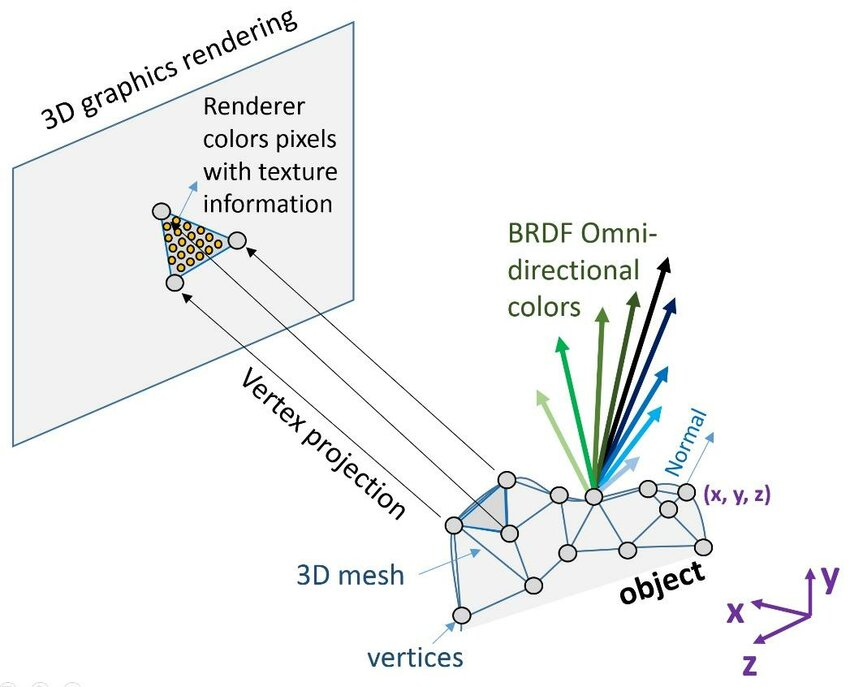
\includegraphics[width=0.8\textwidth]{figures/mesh_rendering.jpg}
    \end{center}
    \caption{Illustration of how a collection of triangles get rasterized onto a screen as demonstrated by Lafruit et al. 2016}
    \label{fig:triangle_rasterization}
\end{figure}

While this approach remains widespread, recent advances in hardware-accelerated ray tracing, particularly with NVIDIA's
RTX series (2018) and AMD's RDNA2 architecture (2020), have enabled real-time ray tracing in commercial applications.
Games like ``Cyberpunk 2077'' and ``Metro Exodus Enhanced Edition'' demonstrate that hybrid approaches combining
rasterization and ray tracing can achieve photorealistic effects such as global illumination and accurate reflections at
interactive frame rates~\cite{keller2019we}. However, both rasterization and ray tracing face similar challenges when
representing highly detailed or volumetric content, leading to the exploration of alternative representations.

Ray tracing functions by ``shooting'' rays out of the camera and into the world, these rays are then tested for
intersections with objects in the world; rays are able to ``bounce'' around in the world, reflect in objects, and cast
shadows. These rays are created in such a way that one, or more, rays are produced for each pixel on the screen that
will allow a given ray to produce a pixel color as seen in Figure~\ref{fig:ray_tracing}.

\begin{figure}[thp]
    \begin{center}
        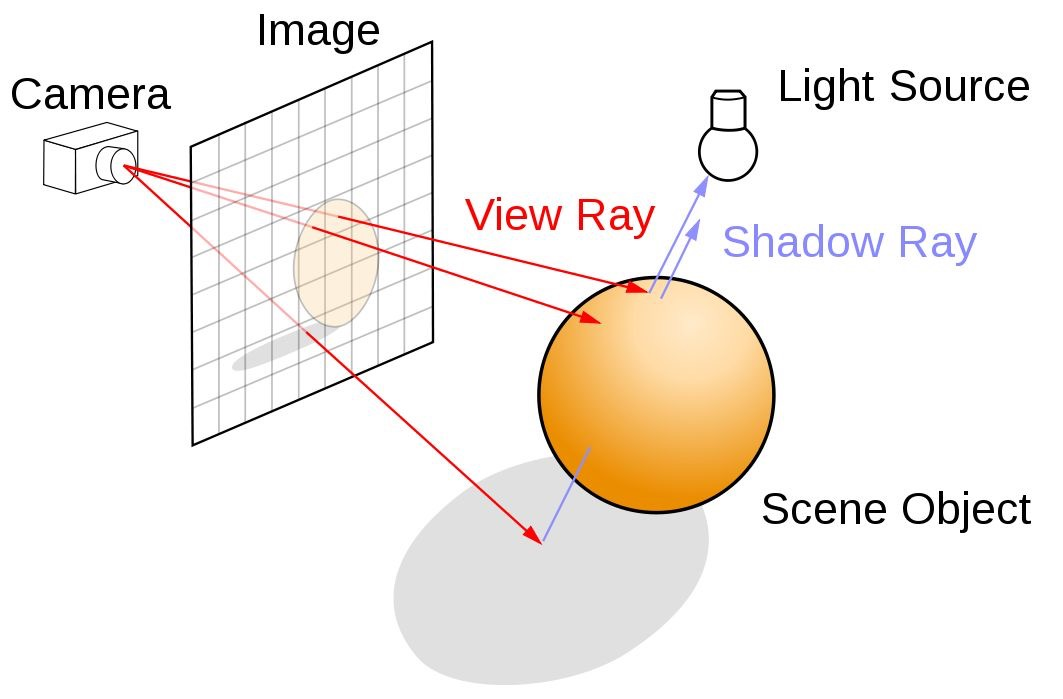
\includegraphics[width=0.8\textwidth]{figures/ray_tracing.jpg}
    \end{center}
    \caption{Visualization of how ray-casting is used to rasterize a 3D world. Source: Wikipedia}
    \label{fig:ray_tracing}
\end{figure}

\section{Voxel-Based Representations and Optimization}

\subsection{Sparse Voxel Octrees}
Sparse Voxel Octrees (SVOs) have emerged as a powerful solution for managing large-scale voxel
worlds~\cite{crassin2009gigavoxels}. Crassin et al.\ (2009) introduced GigaVoxels, a groundbreaking approach that
demonstrated efficient rendering of highly detailed voxel scenes through a hierarchical structure and streaming. Their
work showed that SVOs could effectively compress empty space while maintaining quick traversal times for ray casting.
Building on this foundation, Laine and Karras (2010) developed an efficient sparse voxel octree~\cite{laine2010efficient}
implementation that improved upon previous approaches by introducing a novel node structure and traversal algorithm.
Their method significantly reduced memory requirements while maintaining high rendering performance, making it
particularly suitable for static scenes with complex geometry. Figure~\ref{fig:evso} shows how a 3D voxel world could be
represented as an octree, where the world is recursively divided into smaller and more detailed nodes; only nodes that
encode information are divided into smaller nodes thus saving on memory by not explicitly storing information about
empty nodes at the highest level of detail.

\begin{figure}[thp]
    \begin{center}
        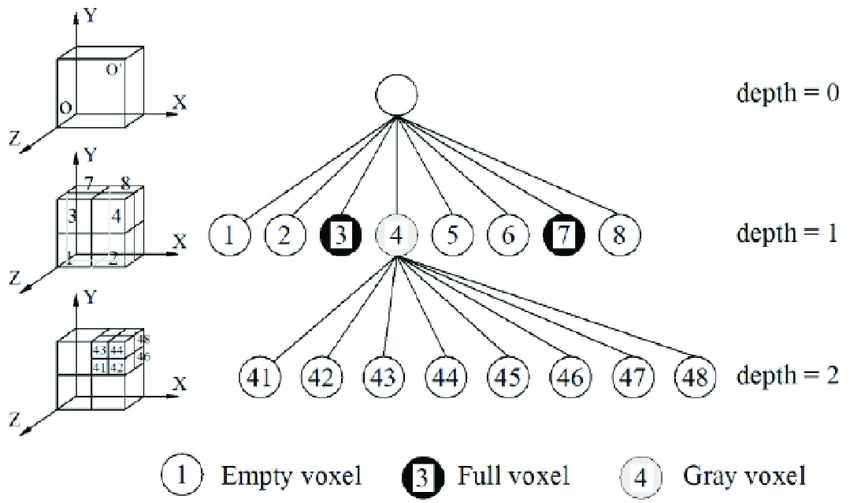
\includegraphics[width=0.8\textwidth]{figures/svo.png}
    \end{center}
    \caption{Illustration of the structure of a Sparse Voxel Octree, nodes with more details have additional
        subdivisions.~\protect\cite{truong2014octree}}
    \label{fig:evso}
\end{figure}

\subsection{Compression and Optimization Techniques}
Several researchers have explored various compression techniques to further optimize voxel storage. Kämpe et al. (2013)
introduced directed acyclic graphs (DAGs) for voxel scenes~\cite{kampe2013high}, achieving compression ratios of up to
50:1 compared to standard SVOs while maintaining real-time rendering capabilities. This approach proved particularly
effective for architectural and synthetic scenes with repeated structures as the repeated structures only needed to be
encoded once with other occurrences only storing references to the encoded structure as can be seen in
Figure~\ref{fig:svdag}

\begin{figure}[thp]
    \begin{center}
        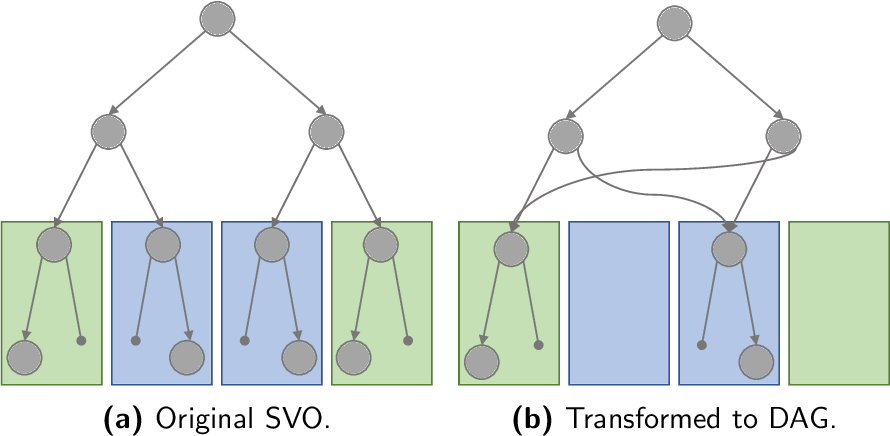
\includegraphics[width=0.8\textwidth]{figures/svdag.png}
    \end{center}
    \caption{Comparison of an octree versus the compressed format of a SVDAG, illustrated as a quad tree for brevity.
        \protect\cite{dolonius2018sparse}}
    \label{fig:svdag}
\end{figure}

\subsection{Challenges in Dynamic Scenes}
The primary challenge in dynamic voxel environments lies in maintaining data structures that can efficiently support
modifications. Updating traditional SVOs in real-time presents significant computational overhead, as changes often
require rebuilding portions of the tree structure. Pan (2021) explored a novel technique for merging SVOs and
dynamically creating nodes where updates are needed~\cite{pan2021dynamic}, while this showcases SVOs have the potential
to support large dynamic scenes, the results show that real-time updates, such as in a video game application, are hard
to achieve.

\section{Distance Fields as an Alternative Representation}
Distance fields have gained attention as an alternative to direct voxel storage, offering several advantages for both
rendering and collision detection. Several recent works have demonstrated the advantages of using distance fields for
real-time rendering of implicit surfaces~\cite{hadji2021raymarching} and function grids~\cite{soderlund2022ray}.
Distance fields are a dense data structure that store the distance to the closest surface for a given point, this can be
seen in Figure~\ref{fig:distance_field}

\begin{figure}[thp]
    \begin{center}
        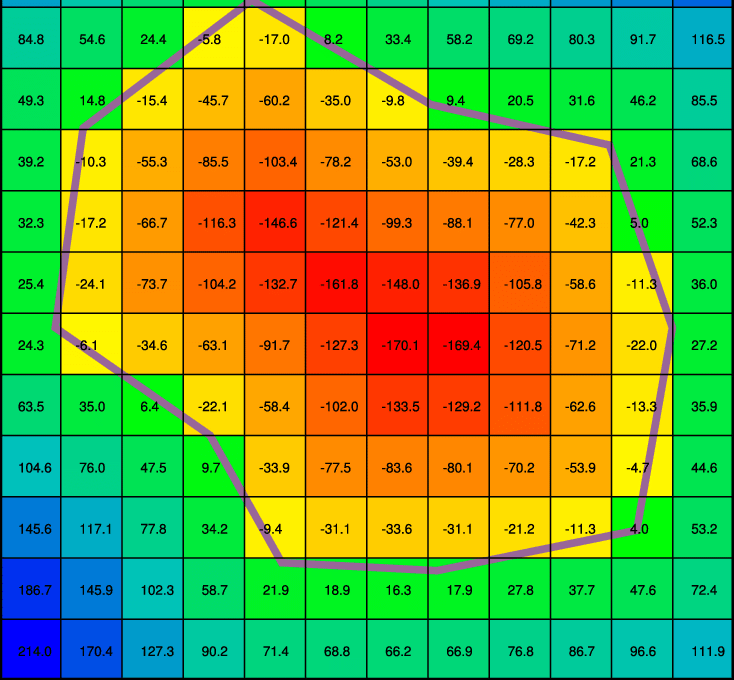
\includegraphics[width=0.8\textwidth]{figures/distance_field.png}
    \end{center}
    \caption{Illustration of a discrete signed distance field grid. Negatives values indicate a cell inside the shape,
        positive values indicate a cell outside the shape.}
    \label{fig:distance_field}
\end{figure}

Ray-marching through a distance field allows you to advance the ray forward by an amount that is guaranteed not to skip
over any features in the world. As seen in Figure~\ref{fig:distance_field_ray_march}, the ray can be advanced in variably
sized steps while ensuring that the ray does not skip through a feature, something that could happen if fixed-size steps
were used.

\begin{figure}[thp]
    \begin{center}
        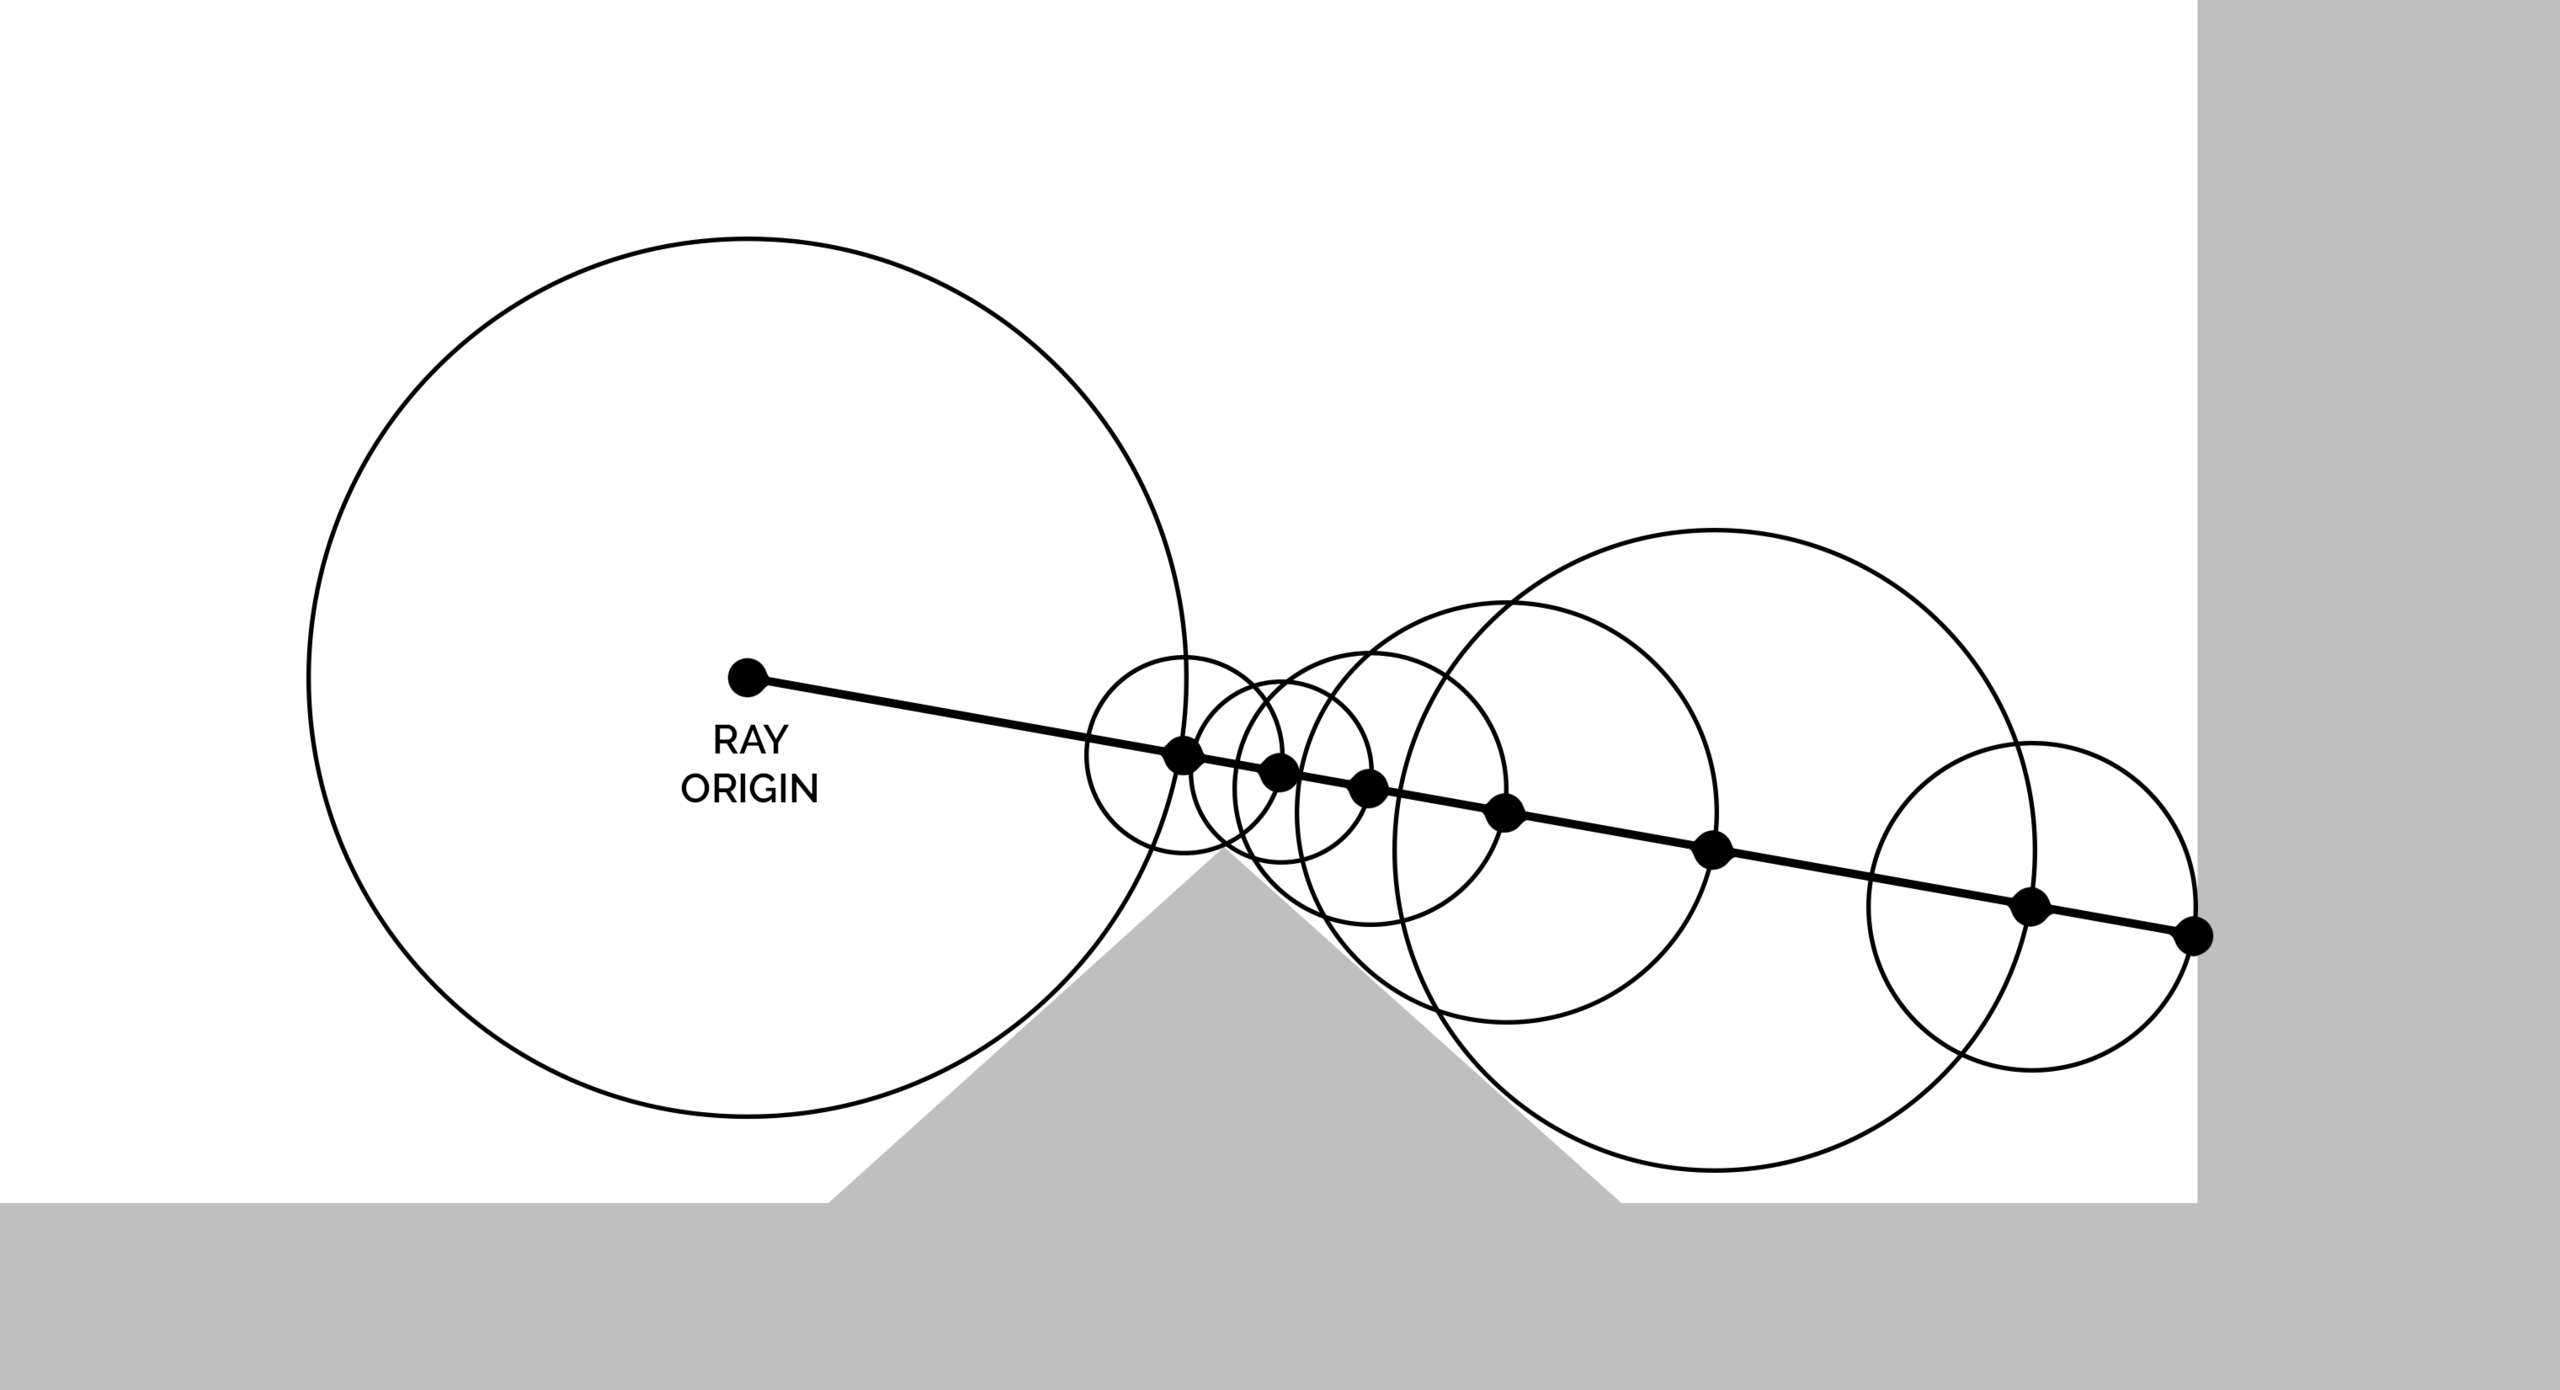
\includegraphics[width=0.8\textwidth]{figures/ray_marching.png}
    \end{center}
    \caption{Illustration of ray marching using a distance field to advance the ray by a variable amount.}
    \label{fig:distance_field_ray_march}
\end{figure}

\subsection{Real-Time Generation and Updates}
The challenge of generating and updating distance fields in real-time remains an active area of research. Techniques
such as Jump Flooding (Rong and Tan, 2006) provide fast approximate solutions but suffer from accuracy
issues~\cite{rong2006jump,rong2007variants}; improvements to Jump Flooding are being researched that allow for it to
be used in dynamic contexts where recalculation of distance fields is needed~\cite{stevenson2022gpu}.
